\section{méthodologie}
La méthodologie est un ensemble de principes utilisées pour guider un processus spécifique. dans notre projet nous  optons pour la methodologie Agile
\subsection{Agile manifesto}
La conduite d'un projet logiciel selon la méthodologie Agile suppose une approche distincte qui privilégie la communication transparente, valorise l'individu et soutient les changements radicaux, tout en favorisant l'auto-organisation des équipes, les incitant à prendre des décisions autonomes et à s'adapter rapidement aux changements.

%\textbf{Manifesto for Agile Software Development }\\
%We are uncovering better ways of developing
%software by doing it and helping others do it.
%Through this work we have come to value:
\begin{enumerate}
    \item  Individuals and interactions over processes and tools
    \item Working software over comprehensive documentation
    \item Customer collaboration over contract negotiation
    \item Responding to change over following a plan 
\end{enumerate}

%That is, while there is value in the items on the right, we value the items on the left more. 

\subsection{Scrum/Agile}
\begin{wrapfigure}{r}{0.25\textwidth} 
    \centering
    
\includegraphics[width=0.25\textwidth]{scrum logo.png}
    \caption{logo de scrum Agile}
\end{wrapfigure}
Selon The Scrum Guide\textsuperscript{\texttrademark}, Scrum est << un framework léger qui aide les personnes, les équipes et les organisations à générer de la valeur grâce à des solutions adaptatives à des problèmes complexes >> Scrum est le framework agile le plus largement utilisé et le plus populaire. Le terme agile décrit un ensemble spécifique de principes et de valeurs fondamentaux pour l'organisation et la gestion d'un travail complexe.
Bien qu'il ait ses racines dans le développement de logiciels, Scrum fait aujourd'hui référence à un cadre léger utilisé dans tous les secteurs pour fournir des produits et services complexes et innovants qui ravissent réellement les clients. C'est simple à comprendre, mais difficile à maîtriser.

\subsubsection{les intervennats}
Scrum compte trois responsabilités (précédemment appelées "rôles") garantissant que chaque aspect du travail partagé est géré de manière efficace.
\begin{enumerate}
    \item \textbf{Développeurs} : Professionnels de l'équipe Scrum qui travaillent ensemble pour créer n'importe quel aspect du produit. Ils créent l'incrément(s) de produit pendant le sprint. Les personnes possédant les compétences nécessaires à la construction du produit assument la responsabilité de développeur. Selon la nature du produit, les compétences seront différentes. 
    \item \textbf{Propriétaire du produit} : Le propriétaire du produit développe et communique l'objectif du produit, possède le backlog du produit et veille à ce que l'équipe s'attaque toujours au travail de la plus haute valeur. Il équilibre également les besoins des parties prenantes, des clients et de l'équipe. Il connaît et comprend le domaine, le marché de ses produits, et il est passionné par la fourniture de résultats que les clients et les utilisateurs veulent et dont ils ont besoin.
    \item \textbf{Maître Scrum} : Le maître Scrum guide et dirige l'organisation dans son adoption et sa pratique du Scrum. Le maître Scrum aide l'équipe à construire le produit et à devenir la meilleure équipe possible en les guidant dans l'utilisation du Scrum et l'incarnation des principes agiles. Il coach l'équipe vers une utilisation efficace des événements et des artefacts. Sa journée peut inclure l'aide à la gestion des obstacles rencontrés par l'équipe, et il est souvent essentiel à la croissance de l'équipe dans son ensemble ainsi que des individus qui la composent.
\end{enumerate}
\subsubsection{la conduite du Scrum Agile}
Il y a cinq événements dans le cadre Scrum. Ces événements sont des occasions précieuses pour inspecter et adapter le produit ou la manière dont l'équipe travaille ensemble (et parfois les deux).
\begin{enumerate}
    \item \textbf{Le sprint} : Au cœur de Scrum, une période limitée dans le temps (moins d'un mois et fréquemment de 1 à 2 semaines) pendant laquelle un ou plusieurs incréments sont créés. Le sprint contient tous les autres événements.
    \item \textbf{Planification de sprint} : L'ensemble de l'équipe Scrum établit l'objectif du sprint. Les développeurs prévoient le travail qu'ils estiment pouvoir accomplir pendant le sprint pour soutenir l'objectif, et comment le travail choisi sera effectué. La planification doit être limitée dans le temps à un maximum de 8 heures pour un sprint d'un mois, avec une durée plus courte pour les sprints plus courts. Sur la base de l'objectif du sprint et des prévisions, un plan initial est également créé. L'équipe Scrum peut inviter d'autres personnes à la planification du sprint pour obtenir des conseils ou des contributions sur le travail pertinent.
    \item \textbf{Scrum quotidien} : Pendant le scrum quotidien, les développeurs inspectent la progression vers l'objectif du sprint et adaptent les plans si nécessaire. C'est un événement quotidien bref dirigé par les développeurs pour inspecter et adapter. Il est limité dans le temps à 15 minutes. Le scrum quotidien n'est pas la seule opportunité pour l'équipe d'adapter ses plans ; elle communique souvent sur les pivots nécessaires en dehors de cet événement. Lors du scrum quotidien, l'équipe peut synchroniser son travail quotidien, identifier les blocages et discuter de la collaboration qui doit avoir lieu. Le scrum quotidien aide l'équipe à comprendre si ses derniers plans les rapprocheront de l'objectif du sprint et à pivoter si nécessaire.
    \item \textbf{Revue de sprint} : L'ensemble de l'équipe Scrum inspecte le résultat du sprint avec les parties prenantes et détermine les adaptations futures. Les parties prenantes sont invitées à donner leur avis sur ce que l'équipe Scrum a accompli jusqu'à présent et sur la direction future du développement du produit. Le backlog du produit est adapté en fonction de ces conversations.
    \item \textbf{Rétrospective de sprint} : La conclusion du sprint, la rétrospective est l'occasion pour l'équipe d'inspecter ses propres interactions, collaborations, processus, outils et tout autre facteur qu'elle juge pertinent pour sa capacité à s'améliorer continuellement.
\end{enumerate}
\cite*{scrumalliance}
\section{téchnologies}

\subsection{Android}
\begin{wrapfigure}{r}{0.25\textwidth} 
    \centering
    
\includegraphics[width=0.25\textwidth]{android-logo.png}
    \caption{logo d'android}
\end{wrapfigure}
Android est un système d'exploitation mobile open source fondé sur le noyau Linux et développé par un consortium d'entreprises, le Open Handset Alliance, sponsorisé par Google. 
Android est défini comme étant une pile de logiciels, c'est-à-dire un ensemble de logiciels destinés à fournir une solution clé en main pour les appareils mobiles, smartphones et tablettes tactiles. Cette pile comporte un système d'exploitation (comprenant un noyau Linux), les applications clés telles que le navigateur web, le téléphone et le carnet d'adresses ainsi que des logiciels intermédiaires entre le système d'exploitation et les applications
\cite*{wiki:Android}

\subsection{Kotlin}
\begin{wrapfigure}{r}{0.25\textwidth} 
    \centering
    
\includegraphics[width=0.25\textwidth]{kotlin.png}
    \caption{logo de Kotlin}
\end{wrapfigure}
Kotlin est un langage de programmation orienté objet et fonctionnel, avec un typage statique qui permet de compiler pour la machine virtuelle Java, JavaScript, et vers plusieurs plateformes en natif (grâce à LLVM). Son développement provient principalement d'une équipe de programmeurs chez JetBrains basée à Saint-Pétersbourg en Russie (son nom vient de l'île de Kotline, près de St. Pétersbourg).
Google annonce pendant la conférence Google I/O 2017 que Kotlin devient le second langage de programmation officiellement pris en charge par Android après Java. Le 8 mai 2019, toujours lors de la conférence Google I/O, Kotlin devient officiellement le langage de programmation voulu et recommandé par le géant américain Google pour le développement des applications Android.
Pivotal Software annonce le 4 janvier 2017 le support officiel de Kotlin sur la cinquième version du Framework Spring. 
\cite*{wiki:Kotlin}
\subsection{les bonnes pratiques}
Dans la documentation Android, on trouve les recommandations ou les "bonnes pratiques" à suivre dans la conception d'une application Android.
\subsubsection{conposition basique d'un logiciel android}
Généralement, un logiciel Android se compose de trois couches fondamentales.
\begin{itemize}
    \item \textbf{couche UI} : consiste à afficher les données de l'application à l'écran. Chaque fois que les données changent, soit à la suite d'une interaction de l'utilisateur (par exemple, si celui-ci appuie sur un bouton) ou d'une entrée externe (telle qu'une réponse du réseau), l'UI doit être mise à jour pour refléter les modifications.
    \item \textbf{couche de domaine} : (facultative) chargée d'encapsuler une logique métier complexe, ou une logique métier simple qui est réutilisée par plusieurs ViewModels.
    \item \textbf{couche de données} : contient la logique métier. La logique métier est ce qui donne de la valeur à votre application. Elle repose sur des règles qui déterminent la manière dont votre application crée, stocke et modifie les données.
\end{itemize}
\begin{center}
    \begin{figure}[h]
        \centering
        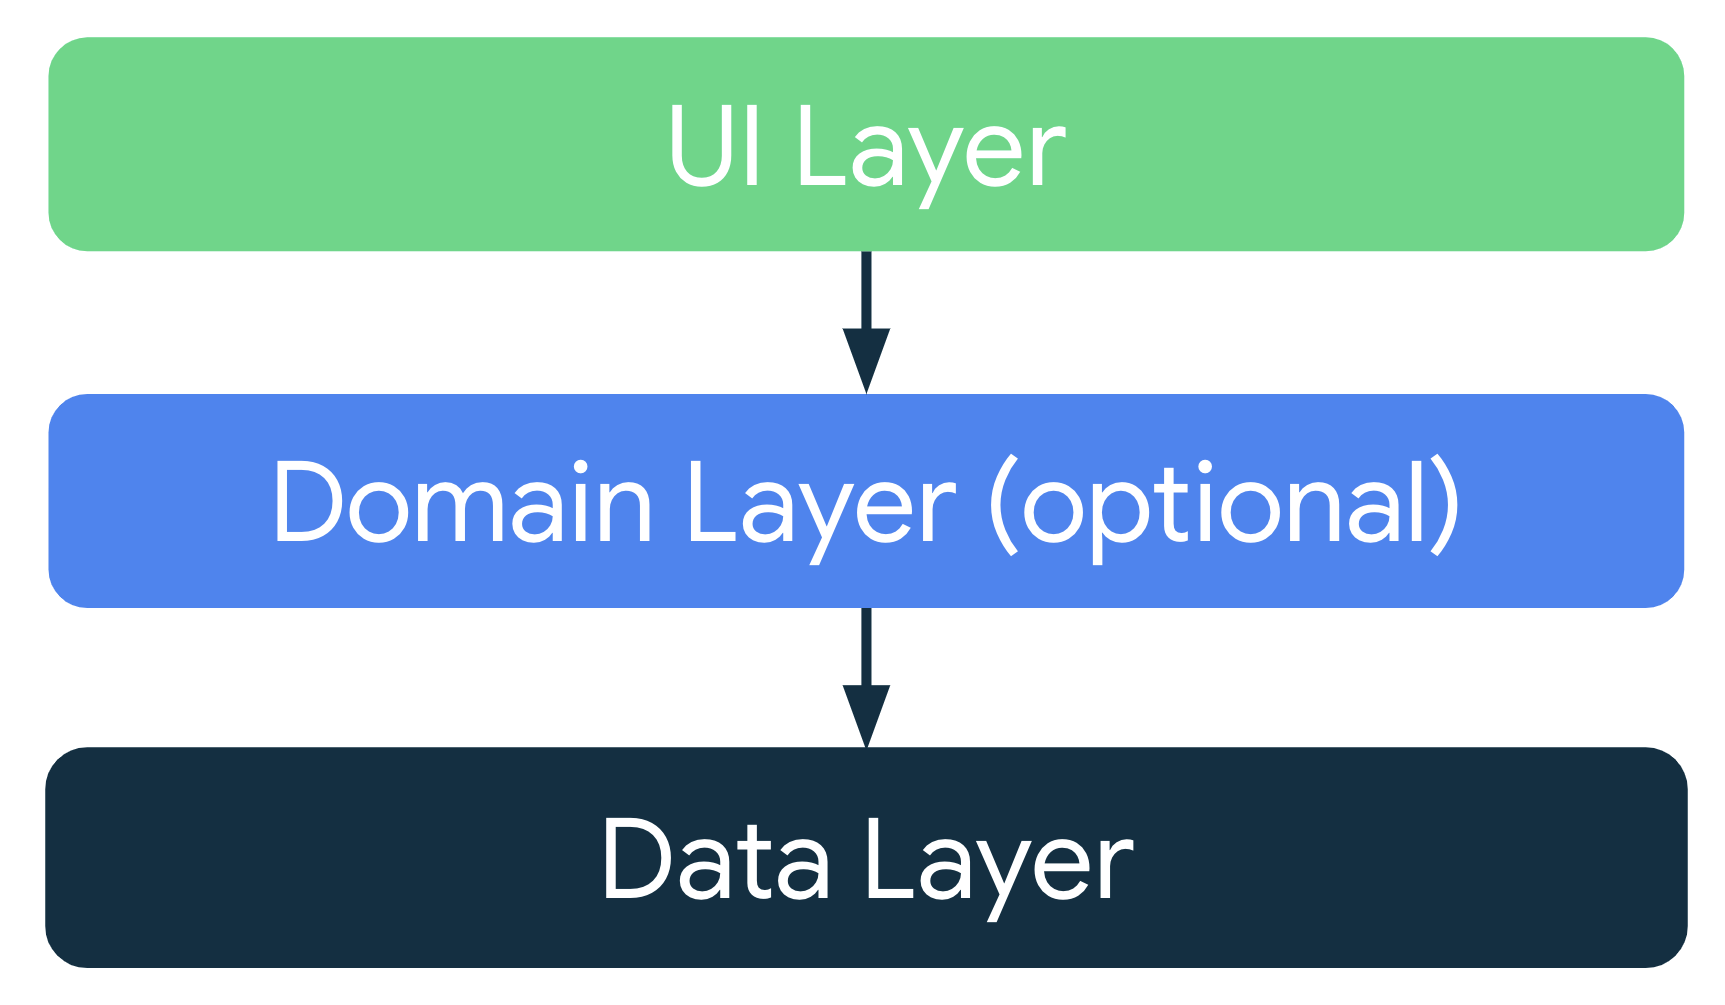
\includegraphics[width=0.5\textwidth]{mad-arch-overview.png}
        \caption{Schéma d'une architecture d'application android} \label{android app schemas}
        \caption*{\small{source : \url{developer.android.com}}}
    \end{figure}
\end{center}
\subsection{Regles a suivre :}
selon le site \url{developer.android.com} il est fortement recommendé de suivre les regles suvantes :
\begin{enumerate}
    \item \textbf{Ne stockez pas de données dans les composants d'une application.}
    \item \textbf{Réduisez les dépendances aux classes Android.}
    \item \textbf{Créez des limites de responsabilité bien définies entre les différents modules de votre application}
    \item \textbf{Exposez le moins d'éléments possible dans chaque module.}
\end{enumerate}
\cite{androidGuideLarchitecture}

\subsubsection{modèle MVVM}
le modele MVVM (Modele-View-ViewModele) est un Design pattern (Modèle de conception) visant à séparer la logique de présentation d'une application en 3 couches 
\begin{enumerate}
    \item \textbf{Model} : Le modèle contient les données liés à la logique métier. Il peut s'agir par exemple d'entités issues de bases de données ou encore d'API externes.
    \item \textbf{View} : La vue est la description de l'interface graphique, elle fait le lien entre les actions de l'utilisateur et le modèle de vue.\\ Elle définie où et comment sont placés les composants graphiques sur l'interface et décris les liaisons de données (Data Bindings) entre les valeurs affichés et le modèle de vue.
    \item \textbf{ViewModel} : Le modèle de vue est chargé de transformer et organiser les modèles métiers afin d'exposer les données à afficher par la vue.
\end{enumerate}
\cite{arkancesystemsQuestPattern}

\subsection{GitHub}
\begin{wrapfigure}{r}{0.25\textwidth} 
    \centering
    
\includegraphics[width=0.25\textwidth]{GitHub-Logo.png}
    \caption{logo de GitHub}
\end{wrapfigure}
GitHub est une plateforme basée sur le cloud  qui offre la possibilité de stocker, partager et collaborer avec d'autres sur l'écriture de code. En stockant le code dans un "référentiel" sur GitHub, vous pouvez :
Suivre et gérer les modifications apportées à votre code au fil du temps.
Permettre à d'autres personnes de réviser votre code et de faire des suggestions pour l'améliorer.
Collaborer sur un projet partagé sans craindre que vos modifications aient un impact sur le travail de vos collaborateurs avant que vous ne soyez prêt à les intégrer

\subsubsection{GitHub Issues}
Le GitHub Issues constituent des entités créées  dans un dépôt pour planifier, discuter et suivre le travail, en assignant des responsabilités, en fixant des priorités et en ajoutant des étiquettes pour classer les problèmes.
Intégrer les GitHub Issues dans notre projet qui adopte la méthodologie agile Scrum offre une organisation transparente du travail, une collaboration efficace et une surveillance stratégique de la progression tout au long du cycle de développement logiciel. Ces Issues servent à représenter les user stories, à assigner des tâches aux membres de l'équipe, suivre l'avancement du travail et discuter des obstacles lors des réunions quotidiennes et des revues de Sprint.
\cite{githubProposGitHub}
\subsubsection{GitHub projects}
GitHub projects propose des fonctionnalités de gestion de projet intégrées qui permettent aux équipes de planifier, organiser et suivre leur travail. Ils offrent une vue visuelle des tâches, des étapes de workflow et des deadlines ls peuvent inclure des Issues, des Pull Requests et d'autres éléments.
Grâce à GitHub Projects, l'avancement de notre travail est surveillée  en temps réel, facilitant ainsi la coordination et la communication au sein de notre équipe. À la fin de chaque Sprint, les données visuelles fournies par GitHub Projects permettent d'examiner le travail accompli et de discuter des améliorations à apporter lors des revues de Sprint et des rétrospectives.
\subsubsection{GitHub Actions}
GitHub Actions est une plateforme d'intégration continue et livraison continue (CI/CD) qui vous permet d'automatiser votre pipeline de génération, de test et de déploiement. Vous pouvez créer des workflows qui créent et testent chaque demande de tirage (pull request) adressée à votre dépôt, ou déployer des demandes de tirage fusionnées en production.
\cite{ComprendreGitHub}

\subsection{Android JetPack Compose}
Jetpack Compose est un kit d'outils moderne conçu pour simplifier le développement des interfaces utilisateur. Il allie un modèle de programmation réactif à la concision et à la facilité d'utilisation du langage de programmation Kotlin.Il est entièrement déclaratif.
%\cite{androidPrincipesBase}

\subsection{Gradle}
%\cite{}
\subsection{Firebase}
Firebase est une plate-forme de développement d'applications et un ensemble d'outils pour l'hébergement, qui permet l'envoi de notifications et de publicités, la remontée des erreurs et des clics effectués dans l'application
%\cite{Firebase}
\subsection{Firebase FireAuth}
Firebase Authentication fournit des services backend, des SDK faciles à utiliser et des bibliothèques d'interface utilisateur prêtes à l'emploi pour authentifier les utilisateurs auprès d'une application. Il prend en charge l'authentification à l'aide de mots de passe, de numéros de téléphone, de fournisseurs d'identité fédérés populaires tels que Google, Facebook et Twitter, etc.
%\cite{Firebase}

TO BE IMPLEMENTED
\subsection{Firebase FireStore}
Cloud Firestore est une base de données flexible et évolutive pour le développement mobile, Web et serveur à partir de Firebase et Google Cloud. Comme Firebase Realtime Database, il maintient les données synchronisées entre les applications clientes via realtime listeners et offre une prise en charge hors ligne pour mobile et Web afin que vous puissiez créer des applications réactives qui fonctionnent quelle que soit la latence du réseau ou la connectivité Internet.
%\cite{Firebase}
\subsection{daggerHilt (injecteur de dependances)}
Hilt est une bibliothèque d'injection de dépendances pour Android qui réduit le code récurrent nécessaire pour injecter manuellement des dépendances dans un projet.Hilt offre une méthode standard pour utiliser l'injection de dépendances dans une application en fournissant des containers pour chaque classe Android du projet et en gérant automatiquement leur cycle de vie. 
Hilt repose sur la bibliothèque d'injection de dépendances Dagger et permet d'intégrer Dagger à une application Android de manière standard.
%\cite{androidInjectionDpendances}

